\section{1174039- Liyana Majdah Rahma}
    \subsection{Teori}
    \begin{enumerate}
        \item {Teks Tokenizer}
        Untuk memudahkan mesin memahami maksud dari apa yang kita inginkan dalam machine learning, kata pada teks disebut token, dan proses vektorisasi dari bentuk kata ke dalam token tersebut disebut tokenizer dan tokenizer akan merubah sebuah teks menjadi simbol, kata, ataupun biner dan bentuk lainnya kedalam token. Dapat dilihat seperti gambar dibawah ini
        \begin{figure}[H]
            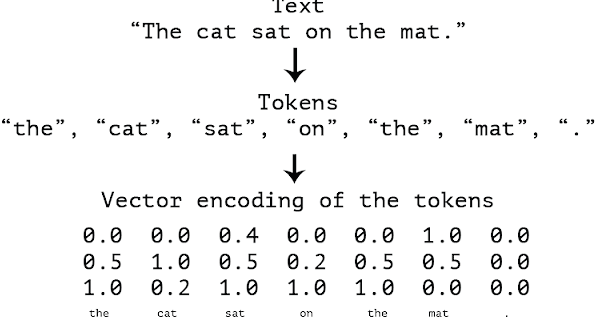
\includegraphics[width=4cm]{figures/1174039/chapter7/1.png}
            \centering
            \caption{Ilustrasi gambar Teks Tokenizer}
        \end{figure}
        
        \item {konsep dasar K Fold Cross Validation pada dataset komentar Youtube} 
        \subitem KStartifiedKFold berisikan presentasi sampel untuk setiap kelas. Dimana dalam ilustrasi ini sampel dibagi menjadi 5 dalam setiap class nya. Kemudian sampel tadi akan dimasukan kedalam class dari dataset youtube tadi. Dapat dilihat seperti gambar dibawah ini
        \begin{figure}[H]
            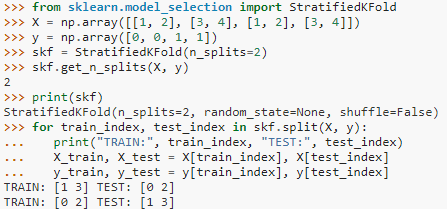
\includegraphics[width=4cm]{figures/1174039/chapter7/2.png}
            \centering
            \caption{Ilustrasi konsep dasar K Fold Cross Validation}
        \end{figure}
        
        \item {kode program for train, test in splits} 
        \subitem Maksudnya yaitu untuk menguji apakah setiap data pada dataset sudah di split dan tidak terjadi penumpukan. Yang dimana maksudnya di setiap class tidak akan muncul id yang sama.  Dapat dilihat seperti gambar dibawah ini
        \begin{figure}[H]
            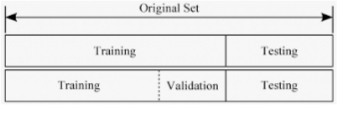
\includegraphics[width=4cm]{figures/1174039/chapter7/3.jpeg}
            \centering
            \caption{Ilustrasi kode program for train, test in splits}
        \end{figure}
        
        \item Jelaskan apa maksudnya kode program \emph{train\_content = d['CONTENT'].iloc[train\_idx]} dan \emph{test\_content = d['CONTENT'].iloc[test\_idx]}. dilengkapi dengan ilustrasi atau gambar}.
        \subitem Maksudnya yaitu mengambil data pada kolom atau index CONTENT yang merupakan bagian dari train\_idx dan test\_idx. Ilustrasinya, ketika data telah diubah menjadi train dan test maka kita dapat memilihnya untuk ditampilkan pada kolom yang diinginkan.
        \begin{figure}[H]
            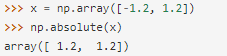
\includegraphics[width=4cm]{figures/1174039/chapter7/4.png}
            \centering
            \caption{Gambar hasil train content}
        \end{figure}
        
        \item Jelaskan apa maksud dari fungsi \emph{tokenizer = Tokenizer(num\_words=2000)} dan \emph{tokenizer.fit\_on\_texts(train\_content)}, dilengkapi dengan ilustrasi atau gambar} 
        \subitem Dimana variabel tokenizer akan melakukan vektorisasi kata menggunakan fungsi Tokenizer yang dimana jumlah kata yang ingin diubah kedalam bentuk token adalah 2000 kata. dan aksudnya kita akan melakukan fit tokenizer hanya untuk dat trainnya saja tidak dengan data test nya untuk kolom CONTENT.Dapat dilihat seperti gambar dibawah ini
        \begin{figure}[H]
            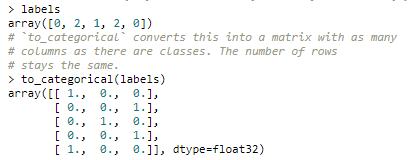
\includegraphics[width=4cm]{figures/1174039/chapter7/5.png}
            \centering
            \caption{Ilustrasi Cara Membaca Hasil Tokenizer}
        \end{figure}
        
        \item {Jelaskan apa maksud dari fungsi \emph{d\_train\_inputs = tokenizer.texts\_to\_matrix(train\_content, mode='tfidf')} dan \emph{d\_test\_inputs = tokenizer.texts\_to\_matrix(test\_content, mode='tfidf')}, dilengkapi dengan ilustrasi kode dan atau gambar} 
        \subitem Maksudnya yaitu untuk variabel d\_train\_inputs akan melakukan tokenizer dari bentuk teks ke matrix dari data train\_content dengan mode matriksnya yaitu tfidf begitu juga dengan variabel d\_test\_inputs untuk data test.Dapat dilihat seperti gambar dibawah ini
        \begin{figure}[H]
            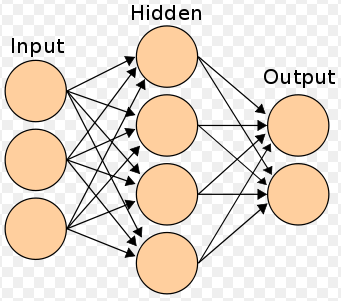
\includegraphics[width=4cm]{figures/1174039/chapter7/6.png}
            \centering
            \caption{Ilustrasi Hasil fungsi train input}
        \end{figure}

        \item {Jelaskan apa maksud dari fungsi \emph{d\_train\_inputs = d\_train\_inputs/np.amax(np.absolute(d\_train\_inputs))} dan \emph{d\_test\_inputs = d\_test\_inputs/np.amax(np.absolute(d\_test\_inputs))}, dilengkapi dengan ilustrasi atau gambar}
        \subitem Fungsi tersebut akan membagi matrix tfidf tadi dengan amax yaitu mengembalikan maksimum array atau maksimum sepanjang sumbu.Dapat dilihat seperti gambar dibawah ini
        \begin{figure}[H]
            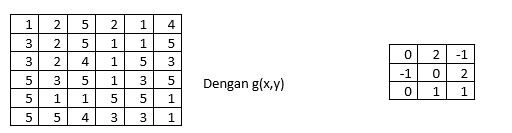
\includegraphics[width=4cm]{figures/1174039/chapter7/7.png}
            \centering
            \caption{Ilustrasi train input dan test input}
        \end{figure}

        \item {Jelaskan apa maksud fungsi dari \emph{d\_train\_outputs = np\_utils.to\_categorical(d['CLASS'].iloc[train\_idx])} dan \emph{d\_test\_outputs = np\_utils.to\_categorical(d['CLASS'].iloc[test\_idx])} dalam kode program, dilengkapi dengan ilustrasi atau gambar}
        \subitem Dalam variabel d\_train\_output dan d\_test\_outputs akan dilakukan one hot encoding, dimana np\_utilsakan mengubah vektor dengan bentuk integer ke matriks kelas biner untuk kolom CLASS dimana nantinya hanya akan ada dua pilihan yaitu 1 atau 0. 1 untuk spam 0 untuk non spam atau sebaliknya.Dapat dilihat seperti gambar dibawah ini
        \begin{figure}[H]
            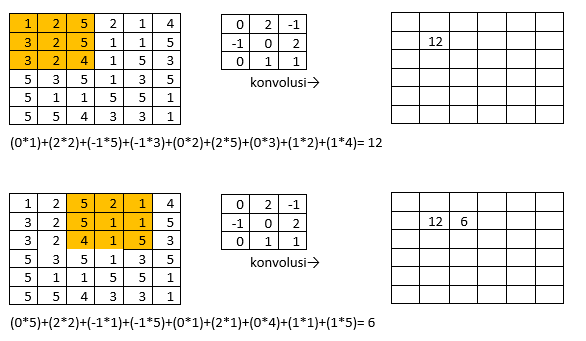
\includegraphics[width=4cm]{figures/1174039/chapter7/8.png}
            \centering
            \caption{Ilustrasi train output}
        \end{figure}

        \item {Jelaskan apa maksud dari fungsi di listing  dilengkapi dengan ilustrasi atau gambar}
        \subitem Melakukan pemodelan Sequential, dan Layer pertama dense dari 512 neuron untuk inputan dengan inputan tadi yang sudah dijadikan matriks sebanyak 2000. Activationnya menggunakan fungsi relu yaitu jika ada inputan dengan nilai maksimum maka inputan itu yang akan terpilih.Dapat dilihat seperti gambar dibawah ini
        \begin{figure}[H]
            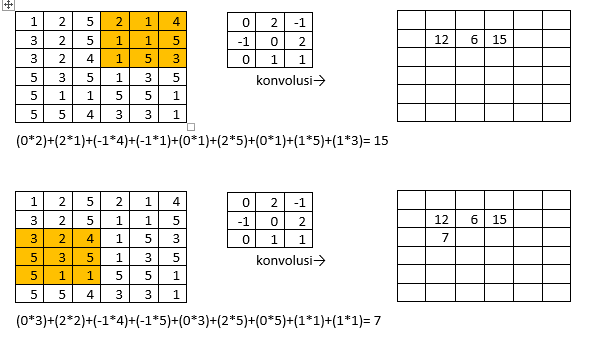
\includegraphics[width=4cm]{figures/1174039/chapter7/9.png}
            \centering
            \caption{Ilustrasi fungsi listing}
        \end{figure}
        \item {Jelaskan apa maksud dari fungsi di listing ke 2 dilengkapi dengan ilustrasi atau gambar}
        \subitem Melakukan peng compile-an dari model Sequential tadi dengan Loss yandengang merupakan fungsi optimisasi skor  menggunakan categorical, dan menggunakan algoritma adam sebagai optimizer. Adam yaitu algoritma pengoptimalan yang dapat digunakan sebagai ganti dari prosedur penurunan gradien stokastik klasik untuk memperbarui bobot jaringan yang berulang berdasarkan data training.Dengan metrik yaitu fungsi yang digunakan untuk menilai kinerja mode Anda disini menggunakan fungsi accuracy.Dapat dilihat seperti gambar dibawah ini
        \begin{figure}[H]
            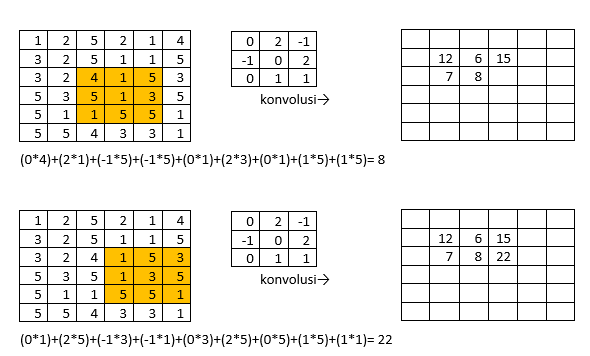
\includegraphics[width=4cm]{figures/1174039/chapter7/10.png}
            \centering
            \caption{Ilustrasi fungsi listing dari model sequential}
        \end{figure}

        \item {Jelaskan apa itu Deep Learning}
        \subitem Deep Learning  adalah subbidang machine learning yang berkaitan dengan algoritma yang terinspirasi oleh struktur dan fungsi otak yang disebut jaringan saraf tiruan atau Artificial Neural Networks. Jaringan saraf tiruan, algoritma yang terinspirasi oleh otak manusia, belajar dari sejumlah besar data. Demikian pula dengan bagaimana kita belajar dari pengalaman, algoritma pembelajaran yang mendalam akan melakukan tugas berulang kali, setiap kali sedikit mengubahnya untuk meningkatkan hasilnya.
            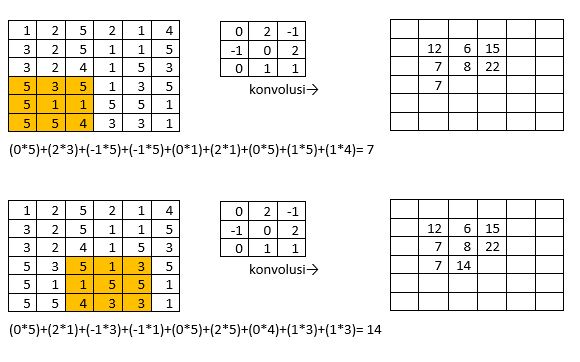
\includegraphics[width=4cm]{figures/1174039/chapter7/11.png}
            \centering
            \caption{pengertian  Deep learning}
        \end{figure}
        \item {Jelaskan apa itu Deep Neural Network, dan apa bedanya dengan Deep Learning}
        \subitem Deep Neural Network adalah jaringan syaraf tiruan (JST) dengan beberapa lapisan antara lapisan input dan output. DNN menemukan manipulasi matematis yang benar untuk mengubah input menjadi output, apakah itu hubungan linear atau hubungan non-linear. Merupakan jaringan syaraf dengan tingkat kompleksitas tertentu, jaringan syaraf dengan lebih dari dua lapisan. Deep Neural Network menggunakan pemodelan matematika yang canggih untuk memproses data dengan cara yang kompleks.
        \begin{figure}[H]
            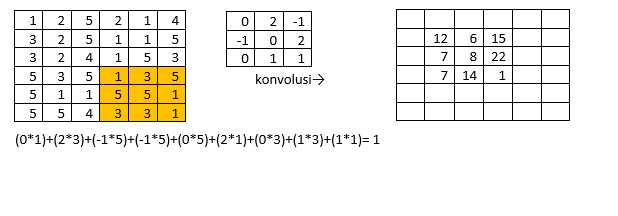
\includegraphics[width=4cm]{figures/1174039/chapter7/12.png}
            \centering
            \caption{perbedaan deep neural network dengan deep learning}
        \end{figure}
        \item {Jelaskan dengan ilustrasi gambar buatan sendiri(langkah per langkah) bagaimana perhitungan algoritma konvolusi dengan ukuran stride (NPM mod3+1) x (NPM mod3+1) yang terdapat max pooling}Stridenya 3
        \subitem Melakukan pemodelan Sequential, dan Layer pertama dense dari 512 neuron untuk inputan dengan inputan tadi yang sudah dijadikan matriks sebanyak 2000. Activationnya menggunakan fungsi relu yaitu jika ada inputan dengan nilai maksimum maka inputan itu yang akan terpilih.Dapat dilihat seperti gambar dibawah ini
        \begin{figure}[H]
            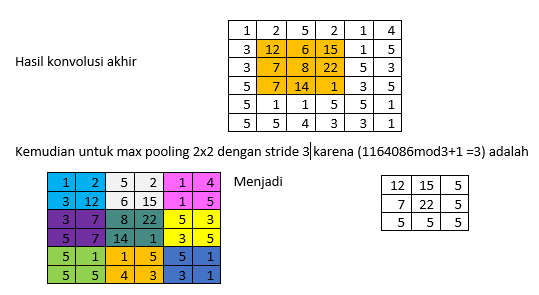
\includegraphics[width=4cm]{figures/1174039/chapter7/13.png}
            \centering
            \caption{Ilustrasi fungsi listing}
        \end{figure}
    \end{enumerate}
    \subsection{Praktek}
        \begin{enumerate}
        \item {No.1 Kode Program Blok In 1}
        \begin{itemize}
        \item Pertama kita akan mengimpor librari csv. Dimana dari librai PIL atau Pillow atau Python Imaging Library akan diimpor modul Image yang di inisiasikan sebagain pil\_image. Modul Image menyediakan kelas dengan nama yang sama yang digunakan untuk mewakili gambar PIL. Modul ini juga menyediakan sejumlah fungsi pabrik, termasuk fungsi untuk memuat image dari file, dan untuk membuat image baru.mengimpor librari image dari keras .Yang menghasilkan kumpulan data gambar tensor dengan augmentasi data waktu nyata. Data akan diulang (dalam batch).Berikut Hasilnya :
        \begin{figure}[H]
            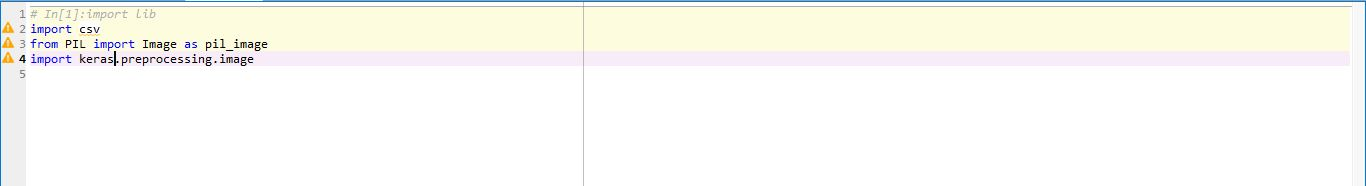
\includegraphics[width=4cm]{figures/1174039/chapter7/praktek1.jpg}
            \centering
            \caption{kode blok satu}
        \end{figure}
        
        \item {No.2 Kode Program Blok In 2}
        \subitem variabel imgs berisikan array kosong
        \subitem  Variabel classes berisikan array kosong
        \subitem Membuka file csv dari Folder HSYv2 dengan nama file hasy-data-labels.csv sebagai csvfile
        \subitem  Variabel csvreader akan menggunakan fungsi reader pada library csv untuk membaca file csv tadi yang disimpan di csvfile.
       \subitem  Dimana variabel i dimuali dari nol.
        \subitem  Untuk setiap baris pada  csvreader
        \subitem  Jika i lebih besar dari 0
        \subitem Jadi itu akan mengambil contoh Gambar PIL dan mengubahnya menjadi array numpy dengan mengambil data dari HSYv2 dan dimulai dari baris ke nol.
        \subitem  Hasil dari variabel img akan dibagi dengan 255.0
        \subitem append akan membuat list array baru untuk baris 0 baris 2 pada img.
        \subitem Menyimpan setiap class nya  pada baris 2
        \subitem  Penambahan i sebanyak 1. 
        \begin{figure}[H]
            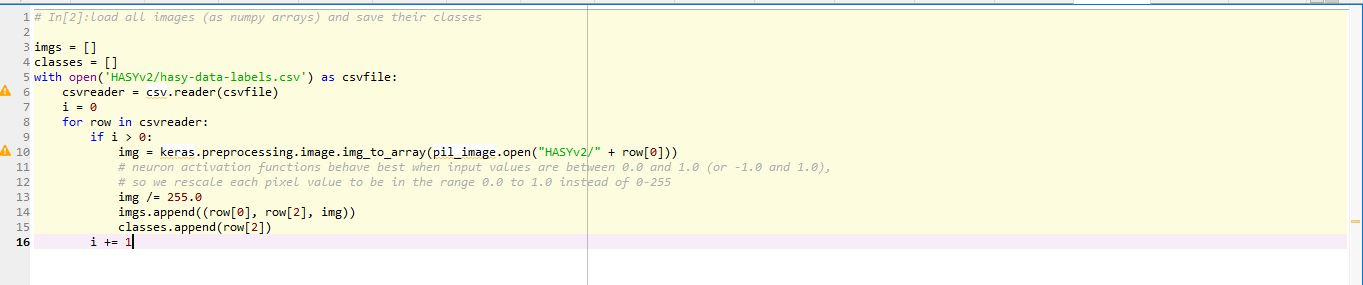
\includegraphics[width=4cm]{figures/1174039/chapter7/praktek2.jpg}
            \centering
            \caption{hasil olah data blok kedua}
        \end{figure}
        
        \item {No.3 Kode Program Blok In 3}
        \subitem  Impor librari Random dari Python
        \subitem  Melakukan pengacakan untuk imgs dengan Metode Shuffle  untuk mengocok urutan di tempat. yaitu, mengubah posisi item dalam daftar.
        \subitem Membagi data dari imgs dengan cara mengalikan 80\% dengan jumlah data dari imgs.
        \subitem  Untuk data train mengambil hasil dari perhitungan sebelumnya.
        \subitem Untuk data test mengambil sisa dari jumlah yang telah dijadikan data train
        \begin{figure}[H]
            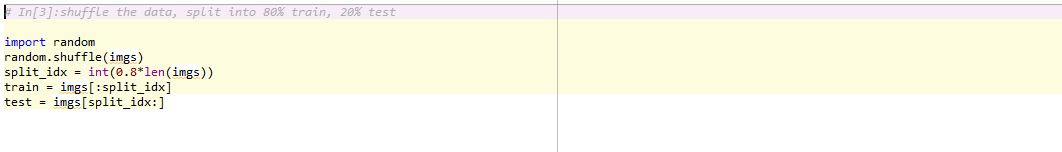
\includegraphics[width=4cm]{figures/1174039/chapter7/praktek3.jpg}
            \centering
            \caption{hasil olah blok in ketiga}
        \end{figure}
        
        \item  {No.4 Kode Program Blok In 4}
        \subitem  Impor librari Numpy yang di inisiasikan sebagai np
        \subitem  Variabel train\_input mengubah input menjadi sebuah array yang diambil dari baris 2, data train.
        \subitem  Variabel test\_input mengubah input menjadi sebuah array yang diambil dari baris 2, data test.
        \subitem  Variabel train\_output mengubah input menjadi sebuah array yang diambil dari baris 1, data train.
        \subitem  Variabel train\_output mengubah input menjadi sebuah array yang diambil dari baris 1, data test.
        \begin{figure}[H]
            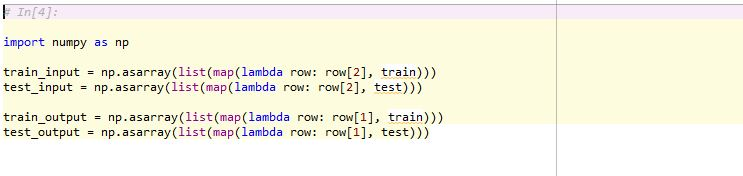
\includegraphics[width=4cm]{figures/1174039/chapter7/praktek4.jpg}
            \centering
            \caption{hasil olah data blok in keempat}
        \end{figure}

        
        \item {No.5 Kode Program Blok In 5}
        \subitem Impor Fungsi LabelEncoder
        \subitem  Impor Fungsi OneHotEncoder
        \begin{figure}[H]
            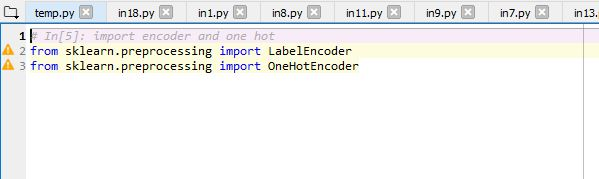
\includegraphics[width=4cm]{figures/1174039/chapter7/praktek5.jpg}
            \centering
            \caption{hasil olah data blok kelima}
        \end{figure}
        
        \item {No.6 Kode Program Blok In 6}
        \subitem Variabel label\_encoder akan memanggil fungsi LabelEncoder tadi.
        \subitem variabel integer\_encoded akan menggunakan labelencoder untuk melakukan fit pada classes agar berubah datanya menjadi integer.
        \begin{figure}[H]
            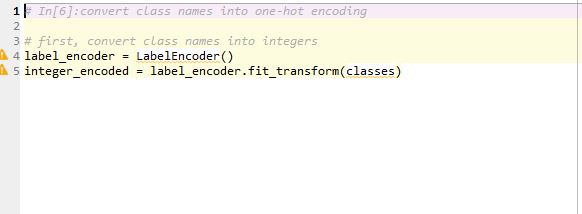
\includegraphics[width=4cm]{figures/1174039/chapter7/praktek6.jpg}
            \centering
            \caption{hasil olah data blok keenam}
        \end{figure}
        
        \item  {No.7 Kode Program Blok In 7}
        \subitem Variabel onehot\_encoder akan memanggil fungsi OneHotEncoder dimana tidak berisikan matriks sparse.
        \subitem  Pada variabel integer\_encoded akan diubah bentuknya dimana setiap nilai integer akan direpresentasikan sebagai vektor binari dengan nilai 0 kecuali index dari integer tersebut ditandai dengan 1.
        \subitem  Melakukan fit untuk one hot encoder kedalam integer\_encoder.
        \begin{figure}[H]
            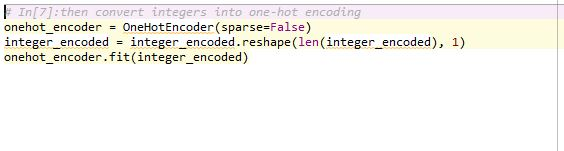
\includegraphics[width=4cm]{figures/1174039/chapter7/praktek7.jpg}
            \centering
            \caption{hasil olah data blok ke tujuh}
        \end{figure}
        
        \item  {No.8 Kode Program Blok In 8}
        \subitem  Variabel train\_output\_int  akan mengubah data dari train\_output menjadi LabeEncoder
        \subitem Variabel test\_output\_int  akan mengubah data dari test\_output menjadi LabeEncoder
        \subitem  Dimana pada train\_output setelah diubah labelnya menjadi integer dilakukan one hot encoding diambil dari test\_output\_int dan menggunakan .reshape untuk memberikan bentuk baru ke array tanpa mengubah datanya dengan keterangan jika index dari integer tersebut ditandai dengan 1 dan sisanya yang bukan nol.
        \subitem  Variabel num\_classes akan menampilakn jumlah data dari classes yang telah dilakukan label encoder
        \subitem  Menampilkan tulisan "Number of classes : \%d dmana mengembalikan nilai integer dari num\_classes.
        \begin{figure}[H]
            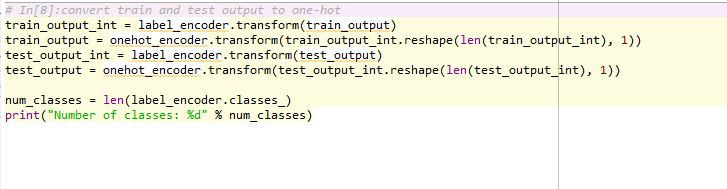
\includegraphics[width=4cm]{figures/1174039/chapter7/praktek8.jpg}
            \centering
            \caption{hasil blok in 8}
        \end{figure}
        
        \item {No.9 Kode Program Blok In 9}
        \subitem Impor Sequential dari model pada librari Keras.
        \subitem Impor Dense, Dropout, Flatten dari modul Layers pada librari Keras.
        \subitem Impor Conv2D, MaxPooling2D dari modul Layers pada librari Keras.
        \begin{figure}[H]
            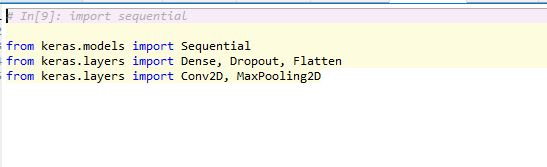
\includegraphics[width=4cm]{figures/1174039/chapter7/praktek9.jpg}
            \centering
            \caption{hasil blok in 9}
        \end{figure}
        
        \item  {No.10 Kode Program Blok In 10}
        \subitem Melakukan pemodelan Sequential.
        \subitem Menambahkan Konvolusi 2D dengan 32 filter konvolusi masing-masing berukuran 3x3 dengan algoritam activation relu dengan data dari train\_input mulai dari baris nol.
        \subitem Menambahkan Max Pooling dengan matriks 2x2.
        \subitem Dilakukan lagi penambahkan Konvolusi 2D dengan 32 filter konvolusi masing-masing berukuran 3x3 dengan algoritam activation relu.
        \subitem Mendefinisikan inputan dengan 1024 neuron dan menggunakan algoritma tanh untuk activationnya.
        \subitem Dropout terdiri dari pengaturan secara acak tingkat pecahan unit input ke 0 pada setiap pembaruan selama waktu pelatihan, yang membantu mencegah overfitting sebesar 50\% .
        \subitem Untuk output layer menggunakan data dari variabel num\_classes dengan fugsi activationnya softmax.
        \subitem Mengonfigurasi proses pembelajaran, yang dilakukan melalui metode compile,sebelum melatih suatu model.
        \subitem Menampilkan atau mencetak representasi ringkasan model yang telah dibuat.
        \begin{figure}[H]
            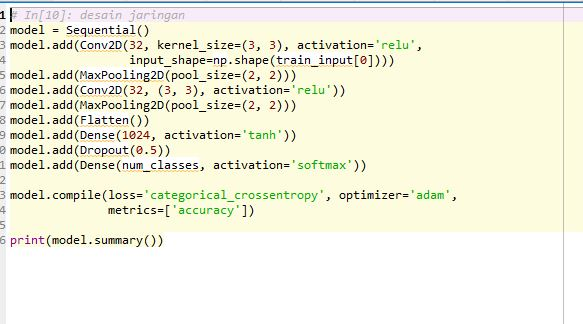
\includegraphics[width=4cm]{figures/1174039/chapter7/praktek10.jpg}
            \centering
            \caption{hasil blok in 10}
        \end{figure}
        
        \item  Impor Modul Callbacks dari Librari Keras.Variabel callback mendefinisikan Callback ini untuk menulis log untuk TensorBoard, yang memungkinkan Anda untuk memvisualisasikan grafik dinamis dari pelatihan dan metrik pengujian Anda, serta histogram aktivasi untuk berbagai lapisan dalam model Anda.
        \begin{figure}[H]
            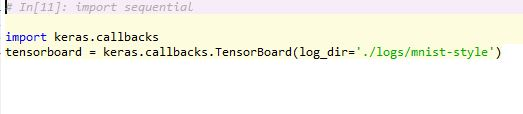
\includegraphics[width=4cm]{figures/1174039/chapter7/praktek11.jpg}
            \centering
            \caption{hasil blok in 11}
        \end{figure}

        \item  Melakukan fit model dengan 32 ukuran subset dari sampel pelatihan Anda Epoch sebanyak 10 kali. Vebrose=2 maksudnya menampilkan nomor dari epoch yang sedang berjalan atau yang sudah dijalankan.Validasi plit sebanayk 20\% sebagai fraksi data pelatihan untuk digunakan sebagai data validasi.Menggunakan TensorBoard sebagai callback untuk diterapkan selama pelatihan dan validasi.Variabel score mengembalikan nilai evaluate untuk menampilkan data lost dan data accuracy dari test yang Menampilkan data loss dengan menghitung jumlah kemunculan nol. Menampilkan data accuracy dengan menghitung jumlah kemunculan 1.
        \begin{figure}[H]
            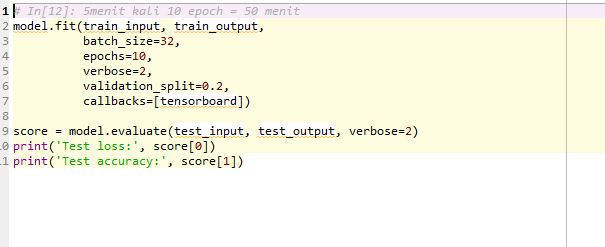
\includegraphics[width=4cm]{figures/1174039/chapter7/praktek12.jpg}
            \centering
            \caption{hasil blok in 12}
        \end{figure}

        \item  impor modul time dari python anaconda. Variabel result berisikan array kosong. Dengan Menggunakan convolution 2D yang dimana akan memiliki 1 atau 2 layer.
        \begin{figure}[H]
            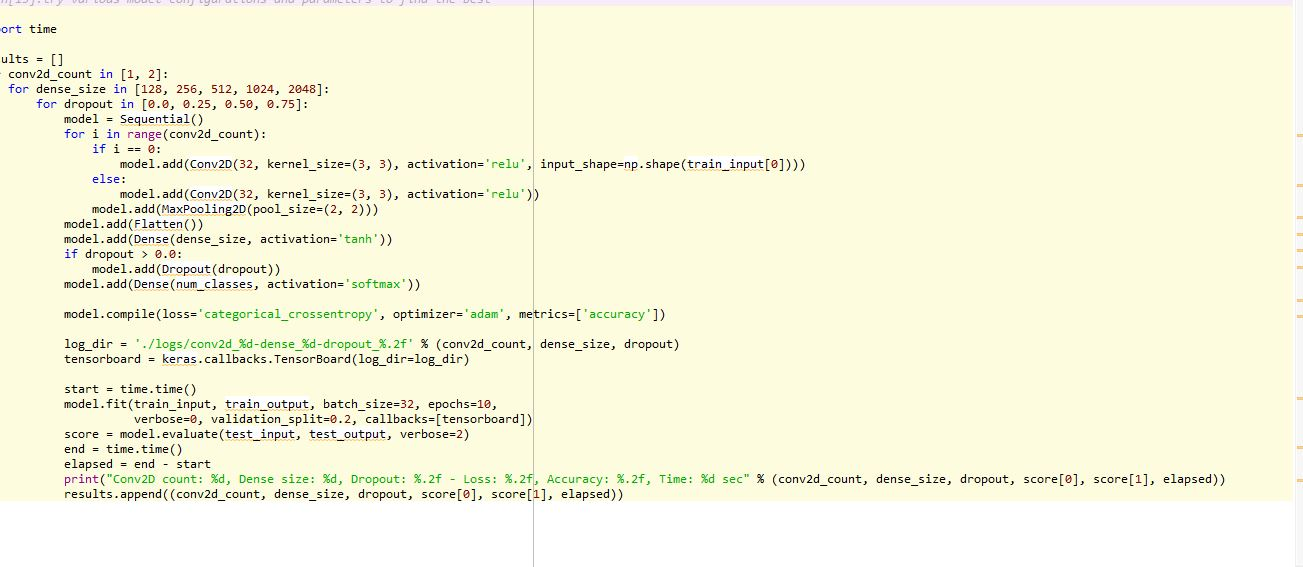
\includegraphics[width=4cm]{figures/1174039/chapter7/praktek13.jpg}
            \centering
            \caption{hasil blok in 13}
        \end{figure}

        \item  Dilakukan Max Pooling 2D dengan ukuran matriks 2x2. Untuk layer kedua, melakukan Convolusi lagi dengan kriteria yang sama tanpa menambahkan input, ini dilakukan untuk mendapatkan data yang terbaik
        \begin{figure}[H]
            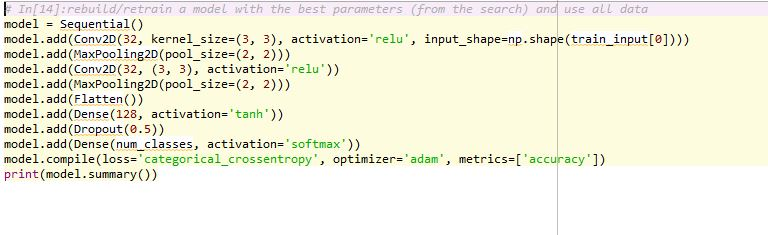
\includegraphics[width=4cm]{figures/1174039/chapter7/praktek14.jpg}
            \centering
            \caption{hasil blok in 14}
        \end{figure}

        \item  I Melakukan fit dengan join data train dan test agar dapat dilakukan pelatihan untuk jaringan pada smeua data yang dimiliki.
        \begin{figure}[H]
            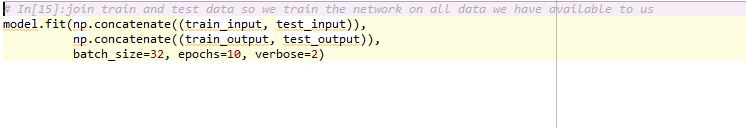
\includegraphics[width=4cm]{figures/1174039/chapter7/praktek15.jpg}
            \centering
            \caption{hasil blok in 15}
        \end{figure}

        \item  Menyimpan atau save model yang telah di latih dengan nama mathsymbols.model 
        \begin{figure}[H]
            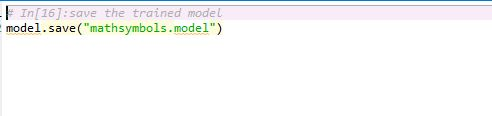
\includegraphics[width=4cm]{figures/1174039/chapter7/praktek16.jpg}
            \centering
            \caption{hasil blok in 16}
        \end{figure}

        \item  Simpan label enkoder.
        \begin{figure}[H]
            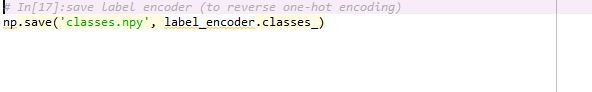
\includegraphics[width=4cm]{figures/1174039/chapter7/praktek17.jpg}
            \centering
            \caption{hasil blok in 17}
        \end{figure}

        \item  Impor models dari librari Keras.Variabel model2 akan memanggil model yang telah disave tadi. kemudian Menampilkan ringkasan dari hasil pemodelan
        \begin{figure}[H]
            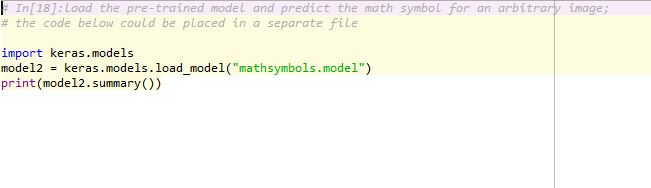
\includegraphics[width=4cm]{figures/1174039/chapter7/praktek18.jpg}
            \centering
            \caption{hasil blok in 18}
        \end{figure}

        \item  Memanggil fungsi LabelEncoder.
        \begin{figure}[H]
            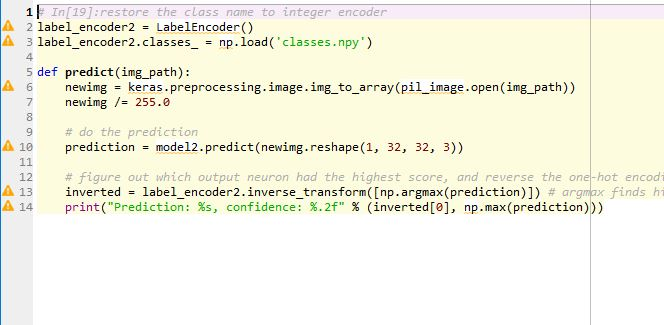
\includegraphics[width=4cm]{figures/1174039/chapter7/praktek19.jpg}
            \centering
            \caption{hasil blok in 19}
        \end{figure}

        \item  Melakukan prediksi dari pelatihan.
        \begin{figure}[H]
            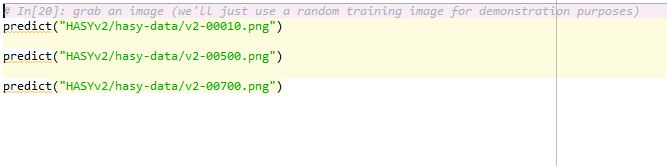
\includegraphics[width=4cm]{figures/1174039/chapter7/praktek20.jpg}
            \centering
            \caption{hasil blok in 20}
        \end{figure}
        \end{enumerate}